\section{Receiver附近确有收益，但找到它的费用也很具体}
四个对象的十二个状态、36个state--budget单元均完成，实际共享current dimension为4、8、16。定向完整复核后的exchange在35个单元有可分辨的完整GN改善，一个单元不变。四对象的汇总风险比中位数为0.348，即完整GN差距下降约65.2\%。这给出了一个明确的正面设计结果：可靠receiver基底只需少量材料相关替换，就能显著改善这一步。对象内先把九个单元的风险相加，再与同一对象的receiver基底比较：
\begin{center}\small\begin{tabular}{@{}lrrr@{}}\toprule
几何 / 材料空间&Local teacher&Verified exchange&Teacher改善取得比例\\\midrule
平滑 / Gaussian&0.0984&0.1904&89.8\%\\
近接触 / Gaussian&0.2016&0.6538&43.4\%\\
分层 / voxel&0.1520&0.2776&85.2\%\\
非对称 / voxel&0.1628&0.4181&69.5\%\\\bottomrule
\end{tabular}\end{center}
前两列是风险比，越小越好。最后一列比较两条最多三个动作的路径各自取得的risk reduction，不是同一checkpoint上的纯评分准确率。Teacher仍须枚举完整声明邻域并支付标签费用。

在每个对象的九个共同receiver checkpoint上，先把单次gain求和再相除，可以更清楚地拆开损失。完整字典anchor top-one的对象级捕获率为98.1--99.6\%，不是每个checkpoint的下界；但十二incoming shortpool只覆盖近接触对象35.3\%的机会，非对称对象65.9\%，平滑和分层对象分别96.9\%、92.0\%。因此，至少在这个共同checkpoint上，近接触对象首先受限于候选覆盖，而不是完整字典内的anchor排名。我没有把不同路径的终点差统统叫作surrogate error。

\begin{figure}[htbp]\centering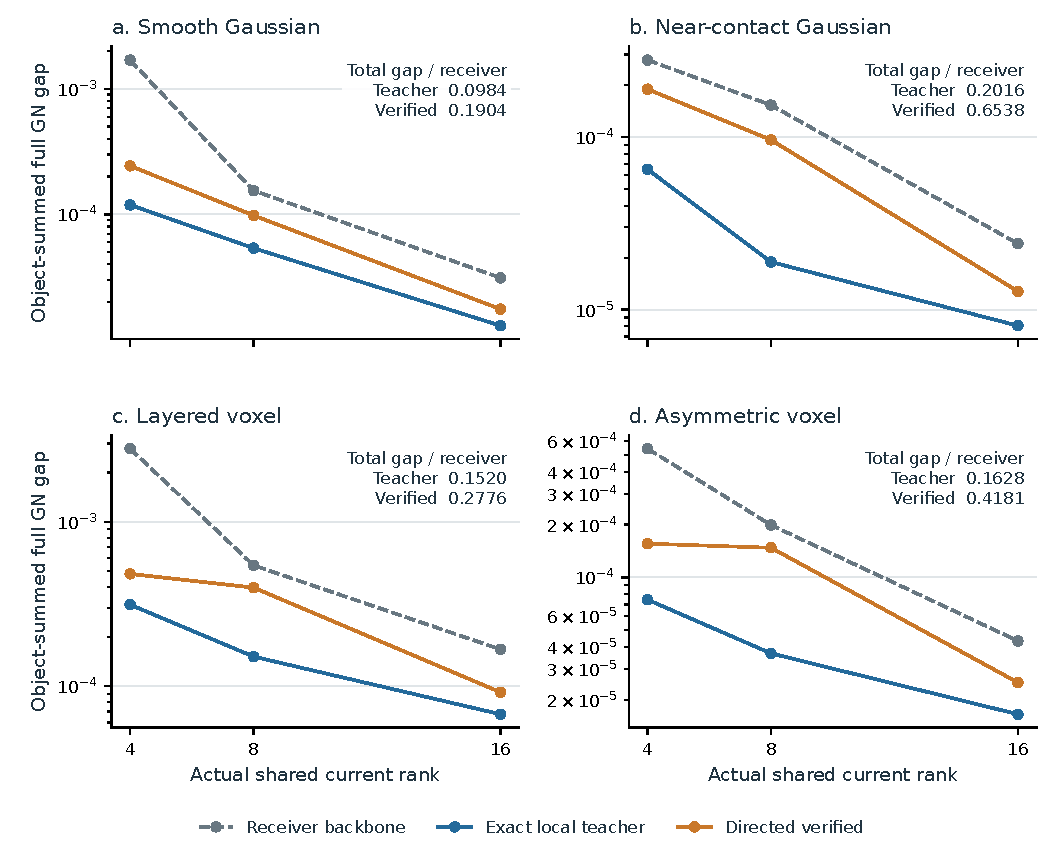
\includegraphics[width=\linewidth]{figures/exchange_risk.pdf}
\caption{三个状态的absolute full-GN gap按对象、current budget汇总。Current teacher只代表声明的局部exchange域；曲线不表示新的nonlinear reconstruction。}
\end{figure}

\section{信息量增加，仍可能把材料步推向错误方向}
我在同一物理材料度量下，将data curvature $\mathsf I_U=J_U^TJ_U$与prior/LM分开。用固定$P=10^{-5}I$归一化后，记录information volume、effective dimension和相对完整曲率的fidelity；voxel仅在十六个共同方向上记录projected diagnostics。这些是固定数值尺度下的局部诊断，没有实测noise covariance支持的互信息解释。

一个近接触对象初始状态的实际交换，使log-det information volume增加6.3127、effective dimension增加1.8613，完整curvature fidelity也略有改善，但actual full gain为$-5.5754\times10^{-5}$。也就是说，一个模型可以声称更多信息，甚至略微改善某个曲率误差指标，却把当前材料步推得更差。这个见证说明information magnitude和该curvature fidelity指标仍不足以决定收益；实际步由residual相关的offset与曲率改变共同决定。这是我认为最需要讲清楚的区别。

另一组common-core测试给出了真实Maxwell相互作用：从rank14开始，分别加一个方向时gain为$-3.2391\times10^{-8}$、$-5.8389\times10^{-8}$，一起加到rank16时变成$3.4787\times10^{-7}$。我将它称为pair interaction witness；它不表示所有greedy方法失效，也不是同秩1-swap局部陷阱。

\section{怎样把这个设计付诸计算，以及接下来需要什么证据}
相同CUDA FP64算子的五次轮换计时中，三个动作上限的conditional selector在近接触Gaussian上为0.594--2.690秒，在分层voxel上为0.891--3.400秒。相同初始shortpool只做一次定向决定为0.328--0.937秒、0.333--1.215秒。公共physical setup与历史anchor/pool acquisition单独计费；这些warm时间没有证明冷启动加速。Receiver不动最便宜；exchange付费换取的是frozen step fidelity。

我也完成了冻结架构的小网络priority pilot，使用对象分组：两个对象训练，一个validation，一个heldout test。MLP的test top-two capture为98.85--99.16\%，group-mean为75.99--98.03\%，都低于已有anchor top-two的99.885\%。特征仍要取得child/anchor信息，fresh physical validation和all-in cost saving没有测得，因此不把这个小试验作为神经选模贡献。

高保真交换检查共接受75个动作，终态22次为信息未解决的abstention、14次达到动作预算。没有合法output-error bound，所以没有严格的acceptance/全邻域停止certificate。允许$\le k$的策略最终仍全部用满$k$，没有取得terminal rank saving。

所有结果首先是full-GN fidelity。无约束$\alpha=1$的一步truth diagnostic相对当前材料，19个单元误差下降、17个上升，28步违反材料约束；它不是line search接受后的重建。Gaussian完整参考在固定prior threshold下也没有full-weak方向；voxel的投影不能断言整个材料空间不弱。我没有据此启动Flow或新的nonlinear reconstruction。

我因此把主线保留为mechanism与conditional local design：材料进入、内部反馈、接收返回共同决定一个模型改动怎样作用；实际是否值得改，还要看offset、curvature、候选覆盖和验证费用。更便宜地识别有用incoming directions，以及把局部gain转成有约束的非线性恢复，仍是最值得进一步弄清楚的部分。
